% Author: Zhenyun Xie

\chapter{Optical Networking Applications Based on Programmable Integrated Photonics}\label{chap:applications_on_pip} % (fold)
% Motivation of this chapter
The hexagonal mesh as one of the most predominant configurations in programmable integrated photonics which enables the recirculation of light to synthesize different photonic circuits.
By properly manipulating PUCs, a dynamic interplay of several optical circuits, such as optical interconnects, splitters, and switches can be programmed.
The conventional control of these programmable circuits consists of tuning each individual PUC sequentially to obtain the desired behavior.
This method requires human intervention, resulting in low efficiency and potential errors.
% Objective of this chapter
In this chapter, graph theory-based routing algorithms are employed to experimentally demonstrate optical networking applications,
such as optical interconnects, optical circuit switching, and optical multicast on a programmable integrated photonic processor.
The corresponding performance metrics are analyzed in detail.

\section{Interconnects}\label{sec:interconnects}
Reconfigurable optical interconnects are of great interest in optical networks as they enable flexible connections of terabit data rates with high-performance operation.
These interconnects demand reduced latency and energy efficiency between input and output (I/O) ports, and therefore minimal insertion loss and shortest distance is highly desired.
The software layer demonstrated herein provides an interconnect algorithm based on Dijkstra, which can automatically provide an optimum path configuration.
This application can also provide self-healing capabilities to allocate alternative optical paths with lower insertion loss when needed.

The results of the optical interconnect experiments at a central wavelength of 1550 nm and the processor configuration are shown in Figure~\ref{fig:ch3-interconnect}.
Ports 0, 37, 17, 6 are used as input ports, and up to 27 interconnects to other available output ports are programmed.
As it can be seen in Figure~\ref{fig:ch3-inter-power}, all the paths are configured successfully, showing diagonal lines in the colormap, each one corresponding to a given interconnect.
The power of the measured output is normalized to the input power of the laser.
The insertion loss at each target port is between 7.7 dB and 10.5 dB, depending on the number of PUCs used to configure the path.
In the experiment, the longest interconnect path consists of 15 PUCs, while the shortest is only 2 PUCs which produces a certain power imbalance between outputs.
Furthermore, optical power is also measured at the rest of the non-targeted output ports, with an average leakage of -30 dB.
The algorithm allows the simultaneous identification of up to 400 possible paths with an average time of about 0.4 microseconds per path.
% figure interconnect
\begin{figure}[h]
    \begin{center}
        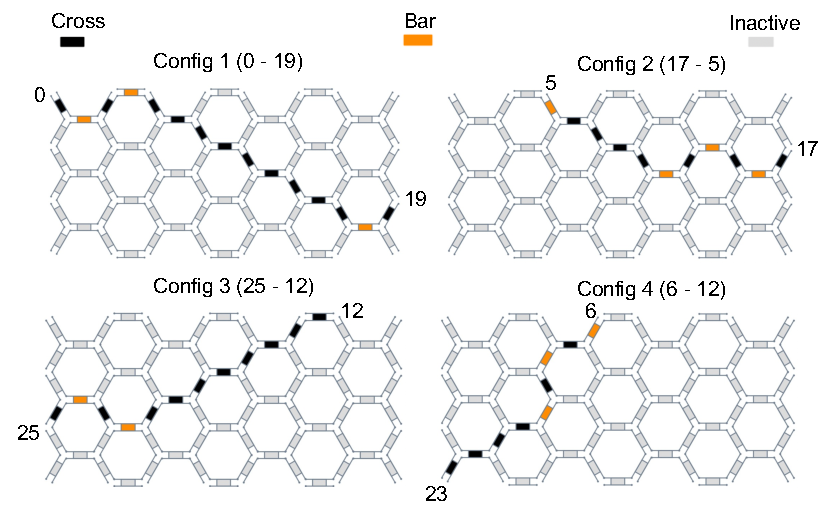
\includegraphics{figures/ch3-interconnect.pdf}
    \end{center}
    \caption{Optical interconnect experiment.
        Programmable processor configurations considering different input ports.
    }\label{fig:ch3-interconnect}
\end{figure}

% figure power interconnect
\begin{figure}[h]
    \begin{center}
        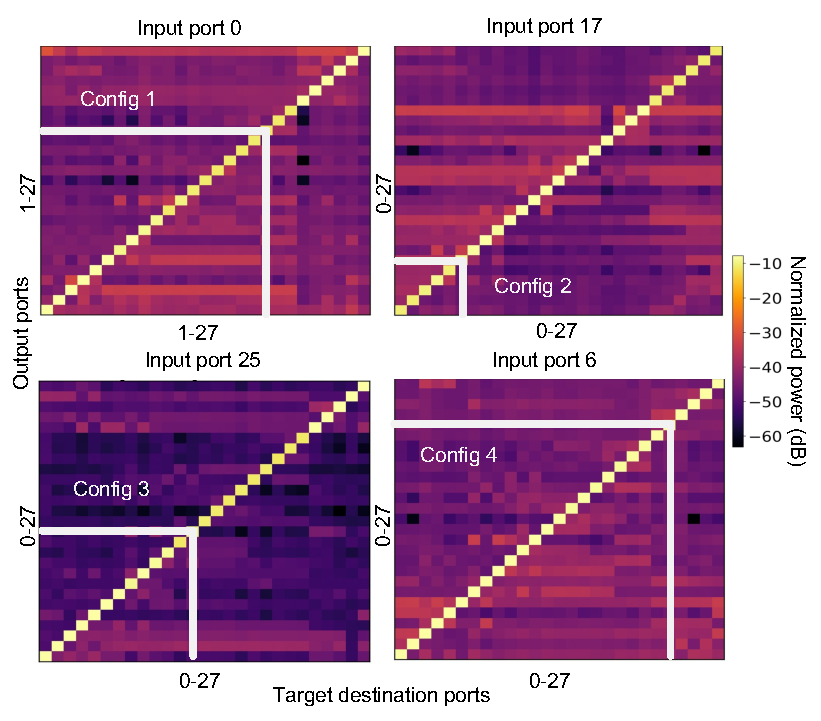
\includegraphics{figures/ch3-inter-power.pdf}
    \end{center}
    \caption{Colormap of the normalized optical power measured at output ports for different interconnect configurations.
        The white lines indicate the configuration shown in the schematic of the programmable processor
    }\label{fig:ch3-inter-power}
\end{figure}

% section Interconnects (end)
\section{Switches}\label{sec:switches}
Optical circuit switching (OCS) is a technology that allows the physical layer of an optical network to be configured through software instructions.
When traffic patterns are predictable and deterministic, OCS allows for direct data routing and topology adjustments entirely within the optical domain.
By eliminating the optical-electrical-optical (OEO) conversion required by traditional Electronic Packet Switches (EPS), OCS significantly reduces latency, power consumption, and operational costs for AI/ML workloads in modern data centers [CITE]
This section demonstrated the implementation of an on-chip software-defined switch designed for the dynamic control of optical waveguide paths for multiple input and output channels.
The system is synthesized on the previously introduced hexagonal core and facilitates a 6x6 cross-connect matrix.
To achieve automated reconfigurability for the full switch matrix, we have adapted three algorithms and implemented them in our software stack.
We have explored three routing algorithms: sequential routing, graph-based edge weight penalty, and analytical decomposition.
The first two are more general as they make use of iterative algorithms to find the non-conflicting routes between the set of port pairs.
Sequential routing is the most computationally intensive, as it exhaustively explores all possible I/O port combinations.
Conversely, the edge weight penalty approach use dynamic graph updates to penalize conflicting path sections.
Once the weight is updated, the routine will attempt to find a new route in the next iteration.
The \textit{max\_iter} parameter (see Algorithm~\ref{alg:auto_switch}) regulates the maximum number of iterations for paths re-routing in instances of edge conflicts, when no routing solution exists for certain input/output port combinations.
Analytical decomposition method offers near instantaneous solutions by mapping the switch matrix to a Spanke-Benes network on a hexagonal mesh.
However, its efficiency is traded for port flexibility, which is constrained by the feed-forward architecture.
Regarding physical performance, the device's reconfiguration is driven by thermo-optic actuators, achieving microsecond-scale (\textit{μs}) switching speeds—orders of magnitude faster than traditional MEMS-based approaches (\textit{ms}).

The fist and the third approaches are straightforward to implement and have been previously documented[CITE].
Here, we document to a deeper extent the second approach that implements the edge penalty algorithm since it offers significantly better
computational efficiency than the brute-force sequential routing of the first approach, while avoiding the ports constraints in the Spanke-Benes architecture.
% algorithm
\begin{algorithm}[htbp]
    \caption{OCS Auto Switch}
    \label{alg:auto_switch}
    \begin{algorithmic}[1]
        \Require $i\_o\_ports$, $\mathit{max\_iter}$, $\mathit{algorithm}$

        \State $preprocessed\_paths \gets \Call{ROUTING\_PREPROCESSING}{i\_o\_ports}$
        \State $best\_paths \gets \emptyset$
        \State $iter \gets 0$

        \While{$iter < \mathit{max\_iter}$}
        \State $conflict\_edges, conflict\_ports \gets \Call{GET\_CONFLICT\_EDGE}{preprocessed\_paths}$

        \If{$conflict\_edges$}
        \State \Call{PENALIZE\_EDGES}{conflict\_edges}
        \State $new\_paths \gets \Call{PATH\_FINDING}{i\_o\_ports}$
        \State $preprocessed\_paths \gets \Call{UPDATE}{preprocessed\_paths, new\_paths}$
        \Else
        \State $best\_paths \gets \Call{GET\_BEST\_PATHS}{preprocessed\_paths, best\_paths}$
        \EndIf

        \State $iter \gets iter + 1$
        \EndWhile


        \If{$best\_paths$ is $\emptyset$}
        \State \textbf{raise} exception
        \EndIf

        \State \Return $best\_paths$
    \end{algorithmic}
\end{algorithm}
% end algorithm




\section{Beamsplitters}\label{sec:beam_splitters}
